\documentclass{beamer}
\usepackage[utf8]{inputenc}
\usepackage[spanish]{babel}
\usepackage{amsmath}
\usepackage{amsfonts}
\usepackage{amssymb}
\usepackage{graphicx}
\usepackage{tikz}
\usetikzlibrary{shapes.geometric}
\usepackage{booktabs}
\usepackage{multirow}

% Tema y configuración
\usetheme{Madrid}
\usecolortheme{default}

% Información del documento
\title{Proyecto Global Integrador: CNC Láser de 3 ejes}
%\subtitle{Aplicación en Brazo Robótico}
\author{Peña Lautaro - Peralta Bruno}
\institute{Universidad Nacional de Cuyo \\ Facultad de Ingeniería \\ Microcontroladores y Electrónica de Potencia}

\setbeamertemplate{footline}{
  \leavevmode%
  \hbox{%
  \begin{beamercolorbox}[wd=.68\paperwidth,ht=2.5ex,dp=1ex,left]{author in head/foot}%
    \usebeamerfont{author in head/foot}Peña Lautaro - Peralta Bruno \hspace{1em} | \hspace{1em} CNC Láser de 3 ejes
  \end{beamercolorbox}%
  \begin{beamercolorbox}[wd=.32\paperwidth,ht=2.5ex,dp=1ex,right]{date in head/foot}%
  \hspace{0.1cm} \insertdate{} \hspace{1cm} \insertframenumber{} / \inserttotalframenumber \hspace{0.1cm}
  \end{beamercolorbox}}%
  \vskip0pt%
}

\begin{document}

% Portada
\frame{\titlepage}


\begin{section}{Introducción}

\begin{frame}
\frametitle{Introducción}
\begin{itemize}
    \item Modificación y reutilización de una impresora 3D antigua para crear una máquina CNC láser.
    \item Destinada a la fabricación rápida de placas de circuito impreso (PCB) para prototipos.
    \item Solución económica y eficiente para proyectos de electrónica y robótica.
    \item Integración de control de motores, programación de microcontroladores y comunicación serial.
    \item Ejecución de comandos G-code para automatizar el proceso de grabado.
\end{itemize}

\end{frame}

\end{section}

\section{Esquema Tecnológico}

\begin{frame}{Esquema Tecnológico}
\begin{center}
\begin{tikzpicture}[node distance=1.2cm, auto]
    % Bloques principales con tamaño reducido
    \tikzset{
        smallblock/.style={
            draw, rectangle, rounded corners, minimum width=2.2cm, minimum height=0.7cm, font=\scriptsize
        }
    }
    \node[smallblock, fill=blue!10] (pc) {PC con G-code};
    \node[smallblock, fill=green!10, below of=pc, yshift=-0.2cm] (bluepill) {Blue Pill STM32F103C8T6};
    \node[smallblock, fill=yellow!20, below of=bluepill, yshift=-0.2cm] (ramp) {RAMPS 1.4};
    \node[smallblock, fill=orange!10, below of=ramp, xshift=-3cm, yshift=-0.2cm] (driverX) {Driver A4988 - Eje X};
    \node[smallblock, fill=orange!10, below of=ramp, xshift=0cm, yshift=-0.2cm] (driverY) {Driver A4988 - Eje Y};
    \node[smallblock, fill=orange!10, below of=ramp, xshift=3cm, yshift=-0.2cm] (driverZ) {Driver A4988 - Eje Z};
    \node[smallblock, fill=red!10, below of=driverX, xshift=-1cm, yshift=-0.2cm] (motorX) {M.PAP NEMA 17HS3430};
    \node[smallblock, fill=red!10, below of=driverY, xshift=0cm, yshift=-0.2cm] (motorY) {M.PAP NEMA 17HS8401};
    \node[smallblock, fill=red!10, below of=driverZ, xshift=1cm, yshift=-0.2cm] (motorZ) {M.PAP NEMA 17HS8401};
    \node[smallblock, fill=gray!20, right of=pc, xshift=2.2cm] (serial) {Monitor Serial};
    \node[smallblock, fill=cyan!20, right of=ramp, xshift=2.7cm] (endstops) {Fines de carrera};

    % Conexiones (con fuente pequeña)
    \draw[-{stealth}] (pc) -- (bluepill) node[midway, left] {\scriptsize USB Serial};
    \draw[-{stealth}] (bluepill) -- (ramp) node[midway, left] {\scriptsize Interfaz};
    \draw[-{stealth}] (ramp) -- (driverX);
    \draw[-{stealth}] (ramp) -- (driverY);
    \draw[-{stealth}] (ramp) -- (driverZ);
    \draw[-{stealth}] (driverX) -- (motorX);
    \draw[-{stealth}] (driverY) -- (motorY);
    \draw[-{stealth}] (driverZ) -- (motorZ);
    \draw[-{stealth}, dashed] (ramp) -- (endstops) node[midway, above] {\scriptsize Sensores};
    \draw[-{stealth}, dashed] (pc) -- (serial);
\end{tikzpicture}
\end{center}
\end{frame}


\section{Diagrama de flujo}

\begin{frame}
\frametitle{Diagrama de flujo}
% Diagrama de flujo del funcionamiento general
\begin{center}
\begin{tikzpicture}[
    scale=0.6,
    transform shape,
    node distance=1.0cm,
    every node/.style={font=\scriptsize},
    process/.style={rectangle, draw, fill=blue!10, rounded corners, minimum width=1.8cm, minimum height=0.5cm, align=center},
    decision/.style={rectangle, draw, fill=yellow!20, minimum width=2.2cm, minimum height=0.8cm, align=center}, % Rectángulo sin esquinas redondeadas
    startstop/.style={rectangle, draw, fill=green!20, rounded corners, minimum width=1.8cm, minimum height=0.5cm, align=center},
    arrow/.style={->, thick}
]

% Nodos (posicionamiento manual, más compactos, distancias ajustadas)
\node[startstop] (start) at (0,0) {Inicio sistema};
\node[process] (init) at (0,-0.9) {Inicializar módulos};
\node[process] (recv) at (0,-1.8) {Recibir G-code desde PC};
\node[process] (interp) at (0,-2.7) {Interpretar comando};
\node[decision] (decision1) at (0,-4.05) {¿Es comando de movimiento?};
\node[process] (action) at (6.4,-4.05) {Ejecutar acción\\(ej: encender láser)};
\node[process] (calc) at (0,-5.4) {Calcular trayectoria\\y pasos de motores};
\node[process] (send) at (0,-6.3) {Enviar señales a drivers};
\node[process] (read) at (0,-7.2) {Leer sensores de límites};
\node[decision] (decision2) at (0,-8.55) {¿Fin de carrera activado?};
\node[process] (stopm) at (-6.4,-8.55) {Detener movimiento};
\node[process] (wait) at (0,-11) {Esperar nuevo comando};
\node[startstop] (error) at (-6.4,-9.9) {Error};

% Flechas
\draw[arrow] (start) -- (init);
\draw[arrow] (init) -- (recv);
\draw[arrow] (recv) -- (interp);
\draw[arrow] (interp) -- (decision1);
\draw[arrow] (decision1) -- node[above]{No} (action);
\draw[arrow] (decision1) -- node[left]{Sí} (calc);
\draw[arrow] (action) |- (wait);
\draw[arrow] (calc) -- (send);
\draw[arrow] (send) -- (read);
\draw[arrow] (read) -- (decision2);
\draw[arrow] (decision2) -- node[above]{Sí} (stopm);
\draw[arrow] (decision2) -- node[right]{No} (wait);
\draw[arrow] (stopm) -- (error);
\draw[arrow] (wait) -- ++(-8,0) |- (interp);

\end{tikzpicture}
\end{center}
\end{frame}


\section{Programacion}
\begin{frame}
    \frametitle{Configuración de Pines}
    \centering
    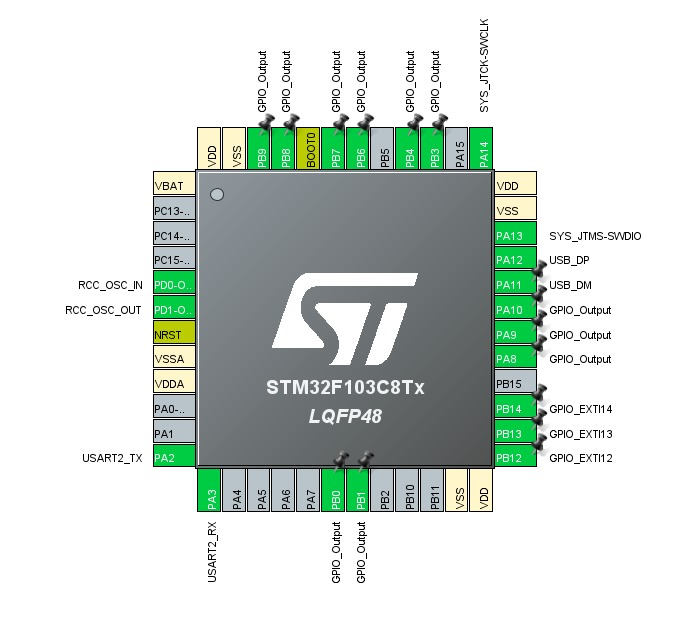
\includegraphics[width=0.7\textwidth]{pines.jpg}
\end{frame}

\begin{frame}
    \frametitle{Configuración de Pines cont.}
\begin{itemize}
    \item \textbf{USB CDC (Communication Device Class):} Comunicación serie virtual via USB, usando los pines PA11 (USB\_DM) y PA12 (USB\_DP).
    \item \textbf{Configuración GPIO para Motores:} 
    \begin{table}[h]
    \centering
    \begin{tabular}{|l|c|c|c|c|}
    \hline
    \textbf{Eje} & \textbf{STEP} & \textbf{DIR} & \textbf{EN} & \textbf{Endstop} \\
    \hline
    X & PB6 & PB7 & PA8 & PB12 \\
    Y & PB9 & PB3 & PB4 & PB13 \\
    Z & PA8 & PA9 & PA10 & PB14 \\
    \hline
    \end{tabular}
    \end{table}
    \item \textbf{Finales de Carrera:} Interrupción por flanco ascendente, utilizando los pines PB12, PB13 y PB14.
    \item \textbf{LEDs de Estado:} Indicador de sistema activo (PB1) e indicador de error (PB0).
\end{itemize}
\end{frame}

\begin{frame}
    \frametitle{Algoritmos de Control de Movimiento}
\textbf{Algoritmo de Bresenham Modificado:} implementado en \texttt{motion.c} para movimientos lineales coordenados.

\begin{itemize}
    \item Cálculo de diferencias absolutas entre coordenadas
    \item Determinación del eje dominante (mayor distancia)
    \item Interpolación lineal para mantener proporcionalidad
\end{itemize}

\textbf{Generación de Arcos:} Algoritmo para movimientos circulares (G2/G3).

\begin{itemize}
    \item División del arco en 50 segmentos lineales
    \item Uso de seno y coseno para interpolación
\end{itemize}

\end{frame}

\begin{frame}
    \frametitle{Parser}
\textbf{Análisis Léxico y Sintáctico:} implementado en \texttt{gcode\_parser.c} con las siguientes características.

\begin{itemize}
    \item \textbf{Parsing modular}: Separación de análisis y ejecución
    \item \textbf{Validación de grupos modales}: Verificación de compatibilidad de comandos
    \item \textbf{Gestión de estado}: Mantenimiento de estado modal persistente
\end{itemize}

\begin{block}{Comandos Soportados}
Los comandos soportados son: \textbf{G0}, \textbf{G1}, \textbf{G2/G3}, \textbf{G28}, \textbf{M114}, \textbf{M119} y \textbf{M503}.
\end{block}
\end{frame}

\begin{frame}
    \frametitle{Ensayos y Validación}

\textbf{Metodología de Pruebas:}
Se implementó un programa de ensayos progresivo utilizando diferentes archivos G-code para validar movimientos básicos, trayectorias complejas y sistemas de seguridad.

\textbf{Resultados Obtenidos:}
\begin{itemize}
    \item \textbf{Velocidades validadas}: 5-60 mm/s sin pérdida de pasos
    \item \textbf{Movimientos 3D}: Coordinación correcta de los 3 ejes
    \item \textbf{Seguridad}: Detección de finales de carrera $<$1ms, homing repetible $\pm 0.01\,\mathrm{mm}$
    \item \textbf{Trayectorias verificadas}: Líneas rectas, círculos y arcos
\end{itemize}

\end{frame}

\begin{frame}
    \frametitle{Conclusiones}
El proyecto cumplió satisfactoriamente con todos los objetivos planteados:

\begin{itemize}
    \item Se desarrolló un sistema CNC funcional basado en STM32F103C8T6
    \item El firmware adaptado de GRBL permite interpretación completa de G-code
    \item La precisión alcanzada es adecuada para las aplicaciones objetivo
\end{itemize}

\begin{block}{Trabajo Futuro}
A futuro podrían implementarse mejoras en:

\begin{itemize}
    \item Hardware
    \item Software
    \item Mecánica
\end{itemize}

\end{block}
\end{frame}

\end{document}